\documentclass[11pt, addpoints]{exam}

\bibliographystyle{abbrv}


\usepackage{pdfpages}
\usepackage{amsfonts}
\usepackage{amsthm}
\usepackage{amssymb}
\usepackage{amsmath}
\usepackage{enumerate}
\usepackage{tikz}
\usepackage{pgfplots}
\usepackage{comment}
\usepackage[margin=1in]{geometry}

%\usepackage{esint}

%\usepackage[all]{xy}

\usepackage{graphicx}

\newcommand{\N}{\mathbb{N}}

\newcommand{\Z}{\mathbb{Z}}

\newcommand{\R}{\mathbb{R}}

\newcommand{\Q}{\mathbb{Q}}

\newcommand{\C}{\mathbb{C}}

\newcommand{\T}{\mathbb{T}}

\newcommand{\ra}{~~\Rightarrow~~}

\newcommand{\lra}{~~\Leftrightarrow~~}

\setlength{\unitlength}{1.5cm}

\addpoints

\begin{document}

\pgfplotsset%Default tikz axis style
{
    width=10cm, height=5cm,
    axis lines=center, 
    grid,
    grid style={very thin, dotted, black!50},
    xmin=-5,    xmax=5,         xtick distance=1,
    ymin=-5,    ymax=5,         ytick distance=1,
    restrict y to domain=-10:10, % <-------
    ticklabel style={font=\scriptsize, fill=white, inner sep=2pt},
    domain=-5:5, samples=100,
    no marks, 
    every axis plot post/.append style={ultra thick, semitransparent,},
}


\section*{Math 241 Practice Midterm 2, Fall 2024}
~\\
~\hspace{2mm}\textbf{Name:}\hspace{2mm}\underline{\hspace{7cm}}\\
~\\
\textbf{Section:}\underline{\hspace{1cm}}\\
~\\
If you do not know your section, fill the following:\\
~\\
\textbf{Instructor:}\underline{\hspace{7cm}}\\
~\\
\textbf{TA:}\underline{\hspace{85mm}}\\

\pagebreak

\begin{questions}

%%%%%%%%%%%%%%%%%%%%%%%%%%%%% Linearization %%%%%%%%%%%%%%%%%%%%%%%%%%%%%%%
\question Let $f(x) = (2x+1)^2$
\addpoints
\begin{parts}
    \part Find the equation of the tangent line of the function $f$ at the point $(2,25)$.
    \vfill
    \part Using your answer in part (a), estimate the value of $(5.1)^2$. Clearly show how you obtain your answer.
    \vfill
\end{parts}
    \pagebreak

\question Use a linear approximation and the fact that $\dfrac{1}{100}=0.01$ to find an approximation to $\dfrac{1}{102}$.
\vfill

\pagebreak

%%%%%%%%%%%%%%%%%%%%%%%% Abs min/max %%%%%%%%%%%%%%%%%%%%%%%%%%%%%%%%%%%%%%%%%
\question Find the absolute min and max of $f(x) = x^2\sqrt{5-2x}$ over the interval $[1, \frac{5}{2}]$

\pagebreak

%%%%%%%%%%%%%%%%%%% Limits at infinity %%%%%%%%%%%%%%%%%%%%%%%%%%%%%%%%%%%%%
\question Compute the following limits. If the limit is $\infty$ or $-\infty$, state which.
\addpoints
\begin{parts}
    \part $\displaystyle\lim_{x\to\infty} \dfrac{-2x^2+3x+1}{7x^2-2}$
    \vfill
    \part $\displaystyle\lim_{x\to -\infty} \dfrac{2x}{x^{2}+7x+6}$
    \vfill
    \part $\displaystyle\lim_{x\to\infty}\, \dfrac{7-4x-x^4}{x^2-22}$
    \vfill
\end{parts}

\pagebreak

%%%%%%%%%%%%%%%%%%%%%%%% Curve shape %%%%%%%%%%%%%%%%%%%%%%%%%%%%%%%%%%%%%
\question Consider the function $f(x) = \dfrac{x^2-4}{x^2+1}$ with the following properties. \textbf{(You do not need to check these properties. In particular, you do not need to differentiate this function).}
\begin{itemize}
    \item $f$ has $x$-intercepts at $x=\pm 2$ and a $y$-intercept at $y=-4$.
    \item $f$ has a horizontal asymptote $y=1$ and no vertical asymptotes.
    \item $f, f',$ and $f''$ are defined for all values of $x$.
    \item $f'(x)$ is negative on $(-\infty,0)$ and positive on $(0,\infty)$.
    \item $f''(x)$ is negative on the open intervals $\left(-\infty,-\frac{1}{\sqrt{3}}\right)$ and $\left(\frac{1}{\sqrt{3}},\infty\right)$. Note that $\frac{1}{\sqrt{3}}\approx .6$
    \item $f''(x)$ is positive on the open interval $\left( -\frac{1}{\sqrt{3}},\frac{1}{\sqrt{3}}\right).$
\end{itemize}
\addpoints
\begin{parts}
    \part Does $f$ have any local extrema? If so, state what type they are and the $x$-value where they occur.
    \vfill
    \part Does the graph of $f$ have any inflection points? If so, give the $x$-coordinate(s).
    \vfill    
    \part Using the information above, sketch the graph of $f$ on the axes below. Clearly mark the horizontal asymptote, $x$ and $y$ intercepts and any inflection points.
    \begin{center}
            \begin{tikzpicture}
                \begin{axis}
                [
                    scale=1.5,
                    xmin=-8.1, xmax=8.1,
                    ymin=-5.1, ymax=2.1,
                    xtick distance=1,
                    ytick distance=1,
                    declare function={f(\x)=\x*\x;}
                ]
                \end{axis}
            \end{tikzpicture}
        \end{center}
%    \begin{center}
%        \includegraphics[width=0.65\textwidth]{Images/Blankgraph.jpeg}
%    \end{center}
\end{parts}
\pagebreak

\question Let $f(x) = 3x^5-5x^3$
\begin{parts}
    \part Find the critical points of $f$
    \vfill
    \part Classify the critical points of $f$ as local maxima, local minima, or neither.
    \vfill
    \part Find the intervals where $f$ is increasing.
    \vfill
    \pagebreak
    \part Find the maximal and minimal values of $f$ on $[-2,0]$.
    \vfill
    \part Find the intervals where $f$ is concave up.
    \vfill
    \part Does $f$ have any inflection points? If so, what are they?
    \vfill
    \part Give a rough sketch of the graph of $y=f(x).$
    \vfill
\end{parts}
\pagebreak

%%%%%%%%%%%%%%%%%% Mean Value Theorem %%%%%%%%%%%%%%%%%%%%%%%%%%%%%%%%%
\question Consider the function $f(x) = \sqrt{2x+1}$ on the interval $[0,3]$.
\addpoints
\begin{parts}
    \part Show that $f$ satisfies the hypotheses of the Mean Value Theorem on the given interval.
    \vfill
    \part Find the value(s) of $c$ in the given interval that are guaranteed by the conclusion of the Mean Value Theorem.
    \vfill
\end{parts}

\pagebreak

%%%%%%%%%%%%%%%%%%%%%%% Optimization %%%%%%%%%%%%%%%%%%%%%%%%%%%%%%%%%

\question A farmer has 600 ft of fencing to enclose a rectangular field along a river which he plans to subdivide into two pens of equal area, with a single length of fencing running down the middle, as in the image below. Notice that he needs no fencing along the river. What is the largest possible area of the field? You need to use calculus to find your solution.
\begin{center}
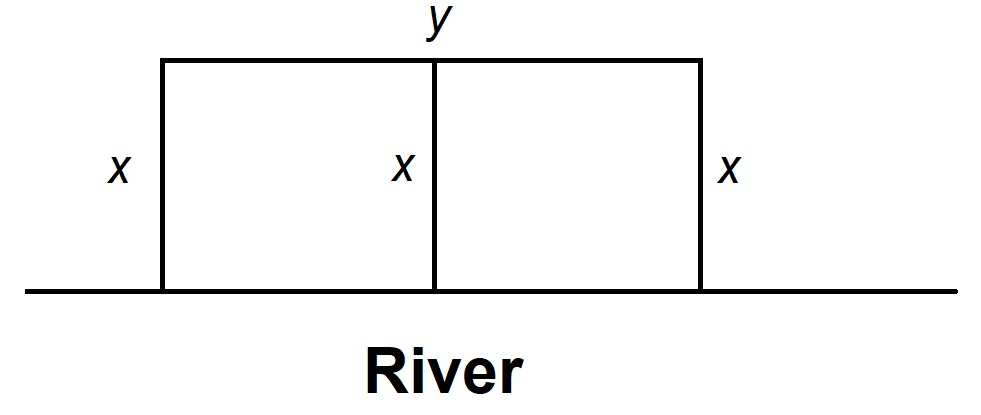
\includegraphics[width=0.35\textwidth]{Images/F23M241MT2MUpic1.jpg}
\end{center}

\pagebreak

\question A rectangular box has a base that is a square. The perimeter of the base plus the height of the box is equal to 3 feet. What is the largest possible volume for such a box, and what are its dimensions? Use Calculus to justify your answer.
\pagebreak

% https://math.libretexts.org/Courses/Mount_Royal_University/MATH_1200%3A_Calculus_for_Scientists_I/3%3A_Applications_of_Derivatives/3.6%3A_Applied_Optimization_Problems

\question A power line needs to be run from a power station located on a beach to an offshore facility underwater located 5000 ft west and 1000 ft north. It costs \$ 50/ ft to run a power line on land and \$ 130/ ft to run the power line under water. How much of the power line should be run along the land to minimize the overall cost? What is the minimal cost?

\begin{center}
    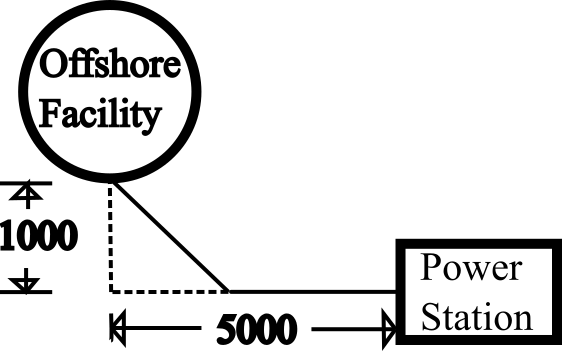
\includegraphics[width=0.35\textwidth]{Images/PMT2drawing.png}
\end{center}

\pagebreak


%%%%%%%%%%%%%%%%%%%%%%%%%% Newton's Method %%%%%%%%%%%%%%%%%%%%%%%%%%%%%%%%%%%%%%%%%%%%%
\question 
\addpoints
\begin{parts}
    \part We wish to estimate the values of $x$ where $\cos(x^{2})=(x+1)^{4}$. What is the appropriate equation to apply Newton's Method to?
    \vfill\vfill
    \part Suppose we wish to approximate the root $Z$ of the function depicted in the following graph. Explain why the x-coordinate of point A is a poor choice for an initial approximation/guess.
    \begin{center}
        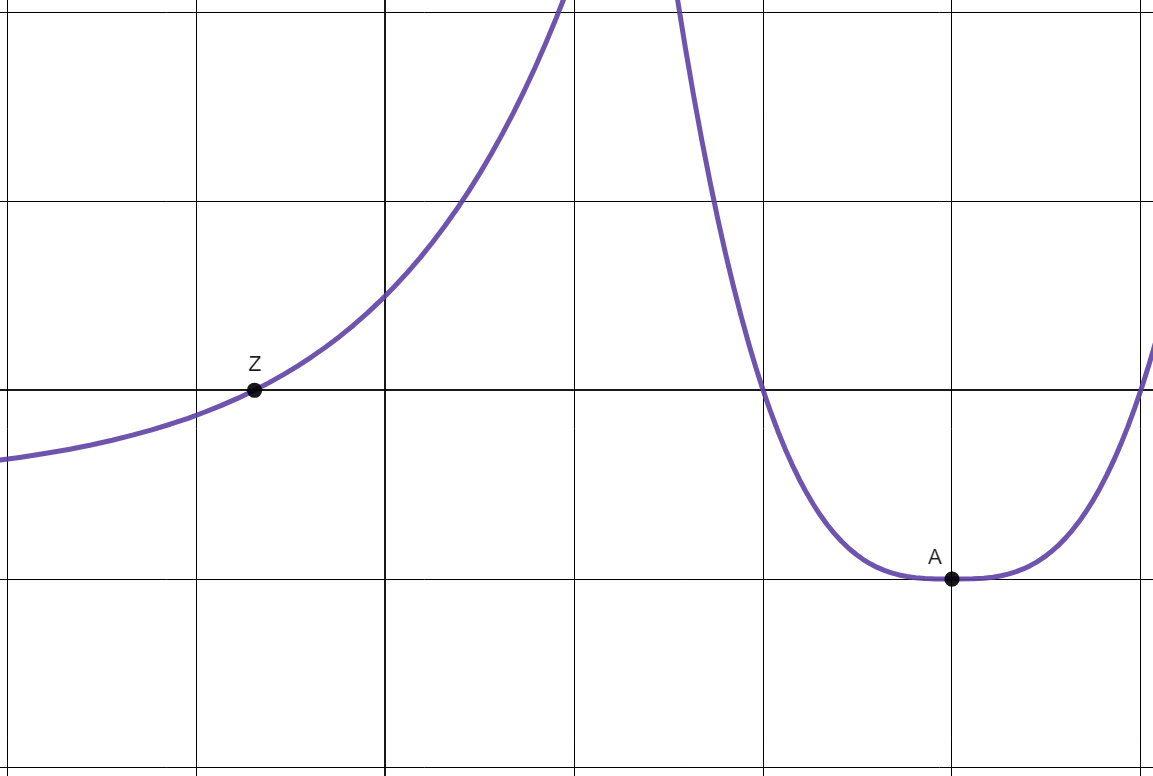
\includegraphics[width=15cm]{Images/1.png}
    \end{center}
    
    \part On the preceding graph, choose an $x$-value, $x_{1}$, which is a good initial approximation and draw $(x_{1},f(x_{1}))$ on the graph. Graphically show how Newton's method is used to generate a second approximation $x_{2}$, and draw and label the point $(x_{2},f(x_{2}))$ on the graph as well as any other geometric attributes pertaining to how you determined $x_{2}$.
    \vfill
    \part For your choice of $x_1$ in the previous part, is $x_2$ greater than or less than the root $Z$?
    \vfill
\end{parts}
\pagebreak

%%%%%%%%%%%%%%%%%%%%%%%%%%%%% Riemann Sums %%%%%%%%%%%%%%%%%%%%%%%%%%%%%%%%%%%%%%%%%%%%%
\question The graph of $f(x) = \dfrac{1}{x-2}$ is given below.
\begin{center}
    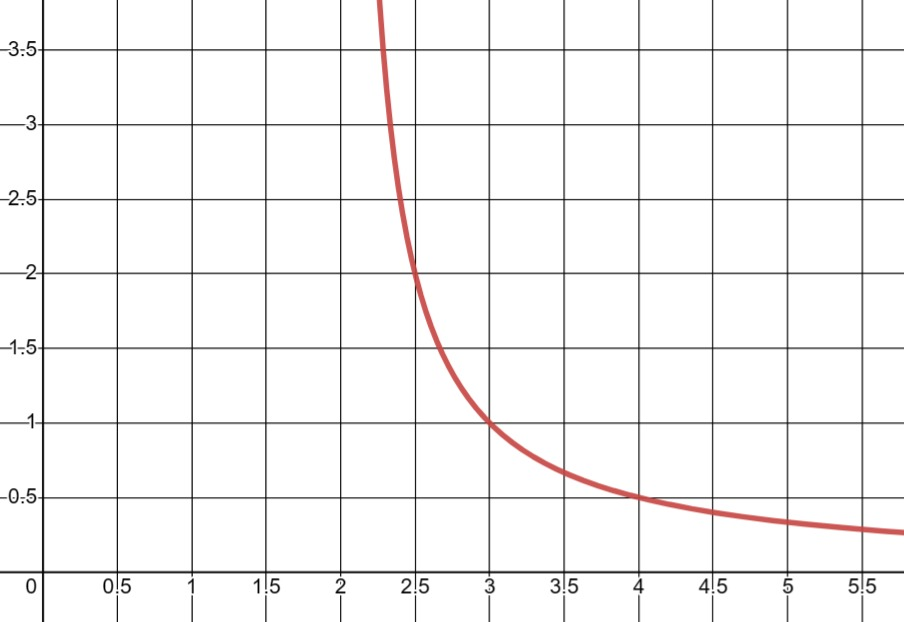
\includegraphics[width=0.75\textwidth]{Images/F23M241MT2MUpic2.jpeg}
\end{center}
\addpoints
\begin{parts}
    \part Estimate $\displaystyle\int_{3}^5 f(x)\,dx$ using four rectangles and right end points.
    \vspace{2in}
    \part Draw the four rectangles from part (a) on the graph above.
    \part Is the estimation in (a) an over or under approximation of the definite integral? Justify your answer.
\end{parts}
\pagebreak

\question Below is the graph of the function $f(x) = -x^2+4$.
\begin{center}
    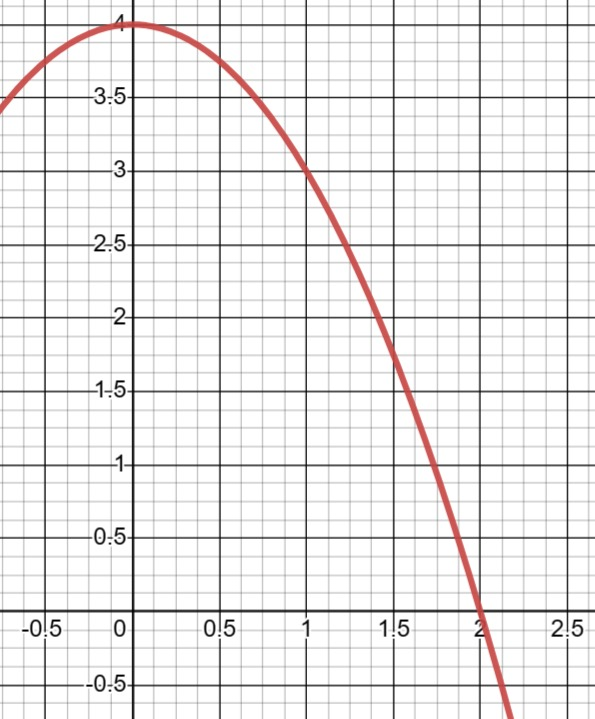
\includegraphics[scale=0.4]{Images/S23 M215 PMT3 pic1.jpeg}
\end{center}

\begin{parts}
    \part Using $n=4$ rectangles with equal bases, approximate the area under the curve of $f(x) = -x^2+4$ over the interval $[0,2]$ using a left end point approximation.
    \vspace{1.5in}

    \part On the graph, draw the four rectangles.
    \part Is your approximation in (a) an overestimate or underestimate of $\int_0^2 f(x)\,dx$? Justify why.
\end{parts}
\pagebreak


%%%%%%%%% QUESTION - Integrals part 2 %%%%%%%%
\question Suppose $f''(x) = 12x - 4$, $f'(2) = 6$ and $f(0) = 1$. Find $f(x).$
\pagebreak

%%%%%%%% QUESTION - AREAS %%%%%%%%%%%

\question Suppose $f$ is continuous on $[a,b]$. What does $\displaystyle\int_a^b f(x)\, dx$ represent?
\vspace{1in}

\question For the graph of $f(x)=\cos(x)$ below, decide which of the following are positive, negative or zero. 

\begin{center}
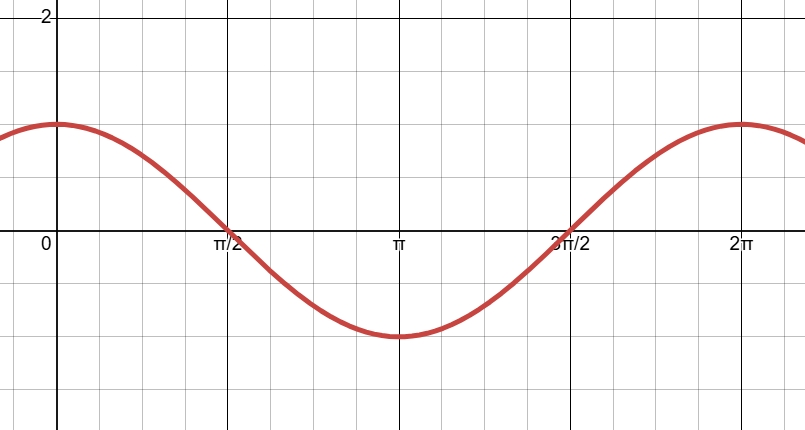
\includegraphics[width=0.75\textwidth]{Images/F24M241 PMT2 pic 1.jpeg}
\end{center}

\begin{parts}
    \part $\displaystyle\int_0^{\pi/2} \cos(x)\, dx$
    \vfill
    \part $\displaystyle\int_{\pi/2}^{3\pi/2} \cos(x)\, dx$
    \vfill
    \part $\displaystyle\int_{3\pi/2}^0 -\cos(x)\, dx$
    \vfill
    \part $\displaystyle\int_{\pi}^{2\pi} \cos(x)\, dx$
\end{parts}

\end{questions}
\end{document}